\section{Features}
In this section we introduce the major features of PureFun. These features include the container types, the type checking and the async feature.
\subsection{Container Types}
The support for the container types list, tuple and map are natively embedded in PureFun. Other than data structures container are mutable.
\subsubsection{List}
Lists are similar to arrays. They contain an arbitrary number of elements sharing the same type.\\
\begin{figure}
\begin{lstlisting}[caption={PureFun code with a list and its predefined functions.},label={ListEx}]
module List {
  list : [Int] = [42,31,69,420]
  fun f () : Void {
    length : Int = #list
    first : Int = list[0]
    newList : [Int] = list ++ [666]
  }
}
\end{lstlisting}
\end{figure}
In listing \ref{ListEx} an example of a list and its predefined functions can be observed. The second line of the listing declares a new global variable named \texttt{list} as a list of \texttt{Int}, which is a 32 bit integer. The variable is instantiated by the list containing the numbers: 42, 31, 69, 420. A list can be instantiated by listing the elements separated by a comma and enclosed by brackets.\\
In line 4-6 the predefined functions are used. The first function using the \texttt{\#} symbol is a short hand notation for the length of a list. The access to individual elements of the list is the same as for the access of array elements in C, using the name of the variable followed by the index in brackets. The last function in line 6 is a short hand notation for the concatenation of two list. In this example the list \texttt{newList} becomes [42,31,69,420,666].\\
PureFun lists are mapped to C++ vectors during the code generation to avoid out of bounds access. Since the size of a list can change, out of bounds access can only be checked during runtime, to avoid large overheads during code generation.
\subsubsection{Tuple}
Tuples are container types, which contain a fixed number of elements. The elements of a tuple do not need to have the same type.\\
Listing \ref{TupleEx} depicts a tuple declaration and its predefined functions. Line 2 declares a tuple with two elements named \texttt{student}, the first element is of type integer and the second one of type string. It is instantiated by the tuple (235212, "Mustermann"). In general a tuple is instantiated by listing the elements enclosed in round brackets.\\
The predefined functions in line 4 and 5 are the same as for the list type. Where the first is a shorthand for the number of elements and the second one is the notation to access a specific element in the tuple.\\
PureFun tuples are mapped to C++ tuples during code generation, for performance reasons and simplicity.
\begin{figure}
\begin{lstlisting}[caption={PureFun code with a tuple and its predefined functions.},label={TupleEx}]
module Tuple {
  student : (Int,String) = (235212, "Mustermann")
  fun f () : Void {
    length : Int = #student
    name : String = student[1]
  }
}
\end{lstlisting}
\end{figure}
\subsubsection{Map}
Maps are a list of key value pairs, where all keys and all values share the same type respectively.\\
Listing \ref{MapEx} shows the declaration and instantiation of a map in PureFun. Similar to the other container types the map \texttt{students} is declared in line 2. The map has keys of type integer and values of type string, which is denoted as [\textit{key}:\textit{value}]. The instantiation is done by listing the key value pairs (\textit{key}:\textit{value}) in curly brackets.\\
The predefined functions in lines 4-7 are defined as follows:
\begin{itemize}
\item \texttt{\#students}: the number of key value pairs.
\item \texttt{students[235212]}: the value corresponding to the key \texttt{235212}
\item \texttt{@students}: the list of all keys
\item \texttt{\$students}: the list of all values
\end{itemize}
PureFun maps are mapped to C++ unordered maps for performance reasons and simplicity.
\begin{figure}
\begin{lstlisting}[caption={PureFun code with a map and its predefined functions.},label={MapEx}]
module Map {
  students : [Int:String] = {235212: "Mustermann", 123456:"Test"}
  fun f () : Void {
    length : Int = #students
    name : String = students[235212]
    keys : [Int] = @students
    values: [String] = $students
  }
}
\end{lstlisting}
\end{figure}
\subsection{Type Checking}

Since we have different types in the PureFun language, it's obligatory to think about implementing type checking in our generator tool. Due to time limitations, we decided to implement type checking partially. We only check primitive types like Int, Strings etc. and our built in container types lists, maps and tuple as well in context conditions. The only types we don't check yet are user-defined data structures defined with the \texttt{data} keyword. We leave the rest of type checking to the C++ compiler.\\
At the time we developed this version of the PureFun language, MontiCore was not capable to generate a rough infrastructure for type resolving. Hence we had to implement the whole type system infrastructure in Java ourselves. Fig. \ref{typeinfrfig1} shows the type infrastructure we implemented in an UML diagram with the most important methods.

\begin{figure}[h]
	\centering
	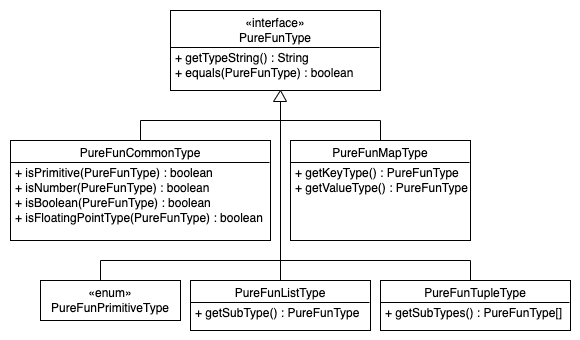
\includegraphics[width=\textwidth]{img/PureFunType.png}
	\caption{PureFun type infrastructure UML diagram}
	\label{typeinfrfig1}
\end{figure}

All types are implementing the PureFunType interface, which provides the methods \texttt{getTypeString()} and \texttt{equals(PureFunType)}. \texttt{getTypeString()} returns the corresponding PureFun type as a \texttt{String}. The PureFunType interface has a default implementation of \texttt{equals} which compares the two type strings with the \texttt{getTypeString} method. This suffices in most cases, but if you think about something like \texttt{var Double = 1}, this \texttt{equals} method would return \texttt{false} for the types of \texttt{var} which is \texttt{"Double"} and \texttt{1} which is an \texttt{Int}. To make this work, we first created the enum \texttt{PureFunPrimitiveType} which contains all primitive types we have in our language. So if we want to extend the primitive datatypes in PureFun with another one, we just have to add it in the \texttt{PureFunPrimitiveType} enum. In addition to the \texttt{PureFunPrimitiveType} enum, we created the class \texttt{PureFunCommonType} which essentially extends the primitive types with the types \texttt{Void} for return values of functions and the type \texttt{Arbitrary} which is mapped to all user-defined types and also the empty list \texttt{[]} for example. The class \texttt{PureFunCommonType} also provides further methods which i.e. can check whether a type is a number type (like \texttt{Int}, \texttt{Float}, \texttt{Double} etc.). With that method we can check whether something like \texttt{var Double = 1} is well typed or not.\\
For lists, we provide the class \texttt{PureFunListType}. Each list has a sub type. The empty list, has the sub type arbitrary, because every list can be instantiated with the empty list. The \texttt{equals} method of \texttt{PureFunType} is overridden here and checks whether sub types of lists are equal or one of them has the arbitrary type.\\
Maps have the \texttt{PureFunMapType} which obviously has a key and a value type. The \texttt{equals} method is overridden here as well like in the \texttt{PureFunListType} class. Here it checks whether key and value type are equal or arbitrary for the empty map.\\
Lastly there is the \texttt{PureFunTupleType} which is similar to \texttt{PureFunListType} but it has multiple sub types. The \texttt{equals} method checks here whether all sub types are equal or if the given tuple type has no subtypes. If the latter is the case, it's the empty tuple.\\
Now that we have our type system infrastructure, we can compare our types. Before we can implement our type checking context conditions, we have to resolve the types. What we get from the AST are only the \texttt{ASTType}s for definitions of variables and functions, \texttt{ASTExpression}s from all the expressions in our language like for example our built in functions for lists and last but not least \texttt{ASTLiteral}s like \texttt{5}, \texttt{31.0}, \texttt{"Hello"} and so on. We have to resolve all the AST classes and map our \texttt{PureFunType}s to them. For that, we created the classes \texttt{PureFunTypeConverter}, \texttt{ExpressionTypesResolver} and \texttt{LiteralTypesResolver}.\\
\texttt{PureFunTypeConverter} has a method \texttt{convertFromAST} which takes an \texttt{ASTType} and returns the corresponding \texttt{PureFunType} object. If the method gets an \texttt{ASTListType} for example, it returns a new \texttt{PureFunListType} object and calls \texttt{convertFromAST} recursively for the sub type. Map and tuple types work analogous. For all other type names, it returns a \texttt{PureFunCommonType} object which has the type name as the type string.\\
\texttt{LiteralTypesResolver} works similar as \texttt{PureFunTypeConverter} but with \texttt{ASTLiteral}. The class provides a method \texttt{resolveType} which takes an \texttt{ASTLiteral} and resolves the type for it corresponding to its subclass. For example if \texttt{resolveType} gets an \texttt{ASTIntLiteral}, then \texttt{resolveType} returns the \texttt{INT} constant from the \texttt{PureFunPrimitiveType} enum. The method works analogous for all other \texttt{ASTLiteral} subclasses.\\
The crucial part of type checking is determining the types of expressions. Consider the assignment expression \texttt{x = calcResult()}. We need to keep two things in mind with that expression. Firstly we need to get the type of the left and the right part in our \texttt{ExpressionTypesResolver}. For that we have to store the types of variables and functions in the symboltable and look it up in the \texttt{ExpressionTypesResolver} which is not a problem with MontiCore. Secondly we need to specify what happens in the resolver if the types do not match (i.e. if \texttt{x} is a \texttt{String} and \texttt{calcResult} has the return type \texttt{Int}). If we return a type in that case, there is no way to check if the expression is well typed in our context conditions. Hence we use the \texttt{Optional} class from Java which allows us to return \texttt{empty} for expressions which are not well typed. For the symboltable MontiCore provides the necessary infrastructure, we simply store the type inferred from the \texttt{ASTType} using our \texttt{PureFunTypeConverter} in \texttt{VariableSymbol} and \texttt{FunctionSymbol}.\\
With this setup we created the \texttt{ExpressionTypesResolver} with a method \texttt{resolveType} which takes an \texttt{ASTExpression} and returns an \texttt{Optional<PureFunType>}. For each expression \texttt{resolveType} calls an internal method matching the subclass of the \texttt{ASTExpression} which resolves the actual type. In our example \texttt{x = calcResult()}, \texttt{resolveType} would call the internal \texttt{doPrintAssignmentExpression} which returns the type of \texttt{x} if the types of the left and right expressions are equal specified by the \texttt{PureFunType} (meaning for example that \texttt{Double = Float} would return true). For the types of \texttt{x} and \texttt{calcResult}, \texttt{resolveType} will be called recursively and calls again internal methods which lookup the return type of \texttt{calcResult} and the type of \texttt{x}. Furthermore if \texttt{calcResult} had parameters, they would have been checked as well.\\
With our type infrastructure, we can now implement all context conditions regarding type checking. As an illustration listing \ref{IfTypeCheckCoco} shows the implementation of type checking on If-Statements. The CoCo is first resolving the type of the condition in an if-Statement using \texttt{ExpressionTypesResolver}. Then it checks if the type is empty (meaning the expression in the condition is not well typed) or if the type is not \texttt{Boolean}. If one of the two cases is true, the user will see an error message with the line number where the type error has occured.

\begin{figure}[h]
\begin{lstlisting}[caption={Implementation of If-Statement type checking CoCo},label={IfTypeCheckCoco}]
public void check(ASTIfStatement node) {
    Optional<PureFunType> conditionType =
       	ExpressionTypesResolver.resolveType(node.getCondition());

    if (!conditionType.isPresent() ||
        	!conditionType.get().equals(PureFunPrimitiveType.BOOLEAN)) {
        Log.error("if condition on line " + 
           node.getCondition().get_SourcePositionStart().getLine() + 
           " has not type Boolean");
        }
}
\end{lstlisting}
\end{figure}

\subsection{Async}
As already mentioned previously the async feature allows the execution with multiple threads without breaking the pureness of the function. Furthermore, async is supported in two different ways:

\begin{enumerate}
\item Async function: a function is called asynchronously.
\item Async block: a set of statements (block) is executed asynchronously.
\end{enumerate}
At the end of this section we introduce some best practices when handling the async feature, since some might increase the runtime of your code.
\subsubsection{Function}
\begin{figure}[h]
\begin{lstlisting}[caption={Example for the async feature on functions.},label={AsyncFun}]
module AsyncFun {
  fun f() : Int {
    left Int = async doSth()
    right Int = doSth()
    return left + right 
  }
}

\end{lstlisting}
\end{figure}
Asynchronous function calls can be used with the keyword async in front of a function call. Listing \ref{AsyncFun} depicts an example for the async on functions. In line 3 the function \texttt{doSth()} is called asynchronously using the async keyword. By utilizing futures from the C++ standard library a new thread is created, which executes \texttt{doSth()} and maps the result to the variable \texttt{left}. Since the function is now executed on another thread the execution of \texttt{f} can continue with line 4. Thus, the call for \texttt{doSth()} in line 3 and 4 can be executed in parallel. This can reduce the overall runtime, if the functions need sufficient time to finish.\\
In line 5 the two partial results \texttt{left} and \texttt{right} are combined to get the result of f. Because the value of left is determined on another thread, we make use of C++ promises to ensure, that all necessary results from different threads are present. If not the execution pauses until all results are present.\\
\subsubsection{Block}
\begin{figure}[h]
\begin{lstlisting}[caption={Example for the async feature on a set of statements (block).},label={AsyncBlock}]
module AsyncBolck {
  fun f() : Int {
    left : Int = 0
    rigth : Int = 0
    async { 
      for i Int = 0; i < genLargeInt(); i++ {
        left = left++ 
      }
    }
    for i Int = 0; i < genLargeInt(); i++ {
      right = right++ 
    }
    return left + right 
  }
}
\end{lstlisting}
\end{figure}
The execution of asynchronous block works similar to the asynchronous functions. The async keyword is used to declare asynchronous execution and the desired block is enclosed in curly brackets. Note that this generates a new scope. Therefore, all variables declared within this block are not available outside of it.\\
In Listing \ref{AsyncBlock} the async block in lines 5-9 executes the enclosed for-loop on a new thread. Similar to the asynchronous functions. Resulting in a parallel execution of both the for-loop in lines 6-8 and the for-loop in lines 10-12. By using the C++ promises it is ensured, that no data races are possible.
\subsubsection{Best Practice}
Parallel execution is generally more complex, than serial execution. This holds both for correctness and runtime predictions for the code. Since data races are covered in chapter 3 on pureness the best practices will focus on the optimization of the runtime. \\
To leverage the async feature appropriately there are a few things to keep in mind:
\begin{itemize}
\item The asynchronous part can overlap with other parts of the execution, e.g. both parts use different variables.
\item The asynchronous part is detached, e.g. it does not need to be evaluated on the spot.
\item The asynchronous part is declared before the part to overlap with.
\item Both the asynchronous part and the part on the main thread are of sufficient runtime to hide the overhead of the thread creation.
\end{itemize}
For example in listing \ref{AsyncFun} the function calls in line 3 and 4 can overlap, because the result is saved in different variables. Furthermore, the result for \texttt{left} is not needed until line 5. The async call for \texttt{left} is declared before line 5, allowing the instantiation of \texttt{left} and \texttt{right} in parallel. At last, if we consider \texttt{doSth()} to be a sufficiently long running function, the runtime of \texttt{f} will be shorter with the async in line 4.\\
By following these best practices most of the overhead induced by the thread creation and the synchronization can be avoided.